As required, we have implemented a simple animation, that starts automatically at the end of execution of Task 3. 

Below, some frames of the animation showing the movement of the quadrotor along the computed optimal trajectory starting from a perturbed initial condition (see task 3): 

\begin{figure}[H]
\centering
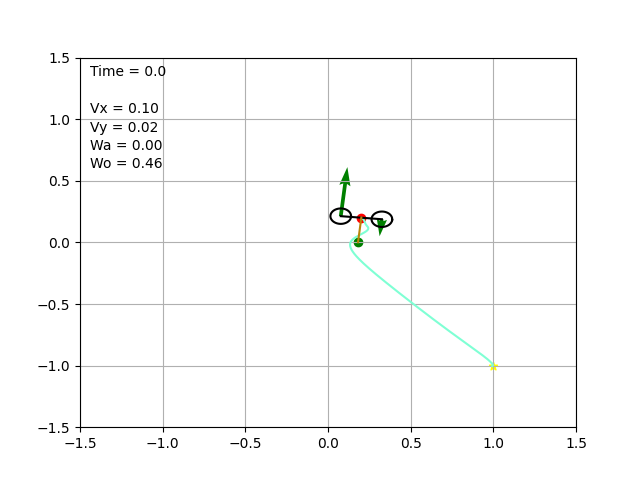
\includegraphics[width=0.9\textwidth]{pictures/ani0.png}
\caption{$t = 0s$}
\label{fig:ani1}
\end{figure}

\begin{figure}[H]
\centering
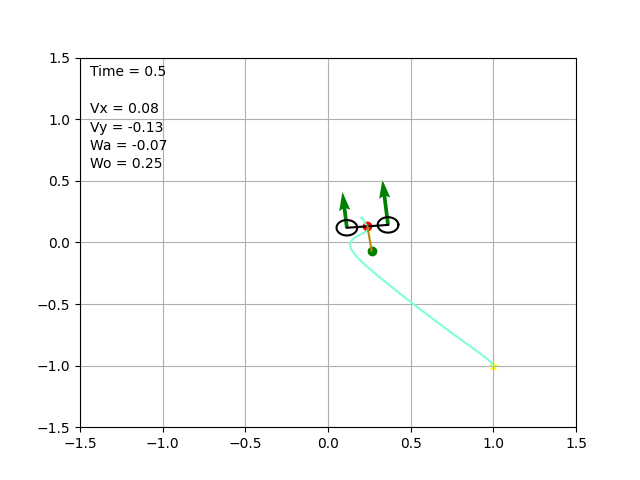
\includegraphics[width=0.9\textwidth]{pictures/ani05.png}
\caption{$t = 0.5s$}
\label{fig:ani05}
\end{figure}

\begin{figure}[H]
\centering
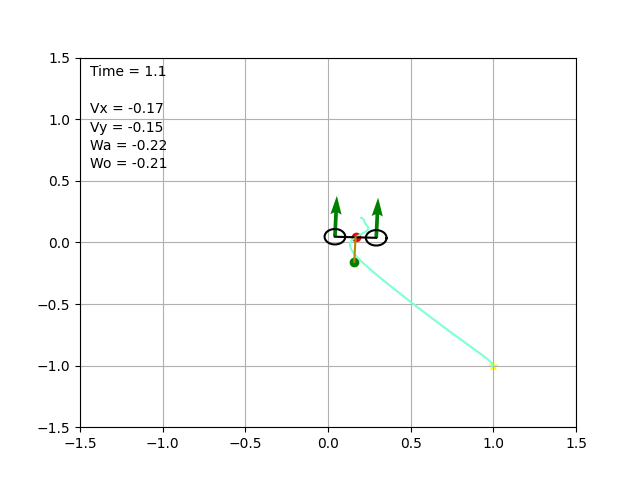
\includegraphics[width=0.9\textwidth]{pictures/ani11.png}
\caption{$t = 1.1s$}
\label{fig:ani11}
\end{figure}

\begin{figure}[H]
\centering
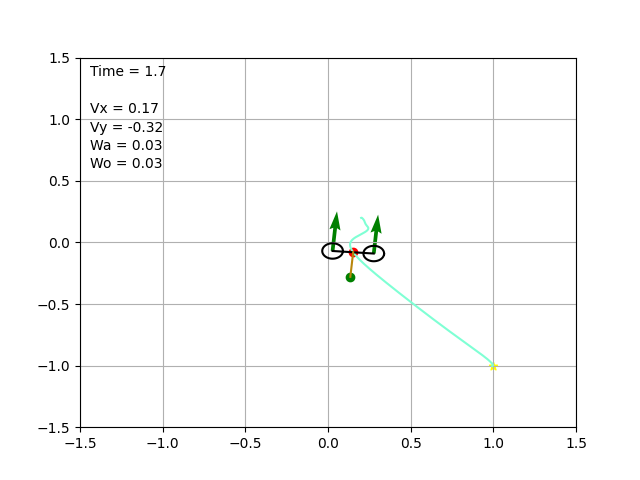
\includegraphics[width=0.9\textwidth]{pictures/ani17.png}
\caption{$t = 1.7s$}
\label{fig:ani17}
\end{figure}

\begin{figure}[H]
\centering
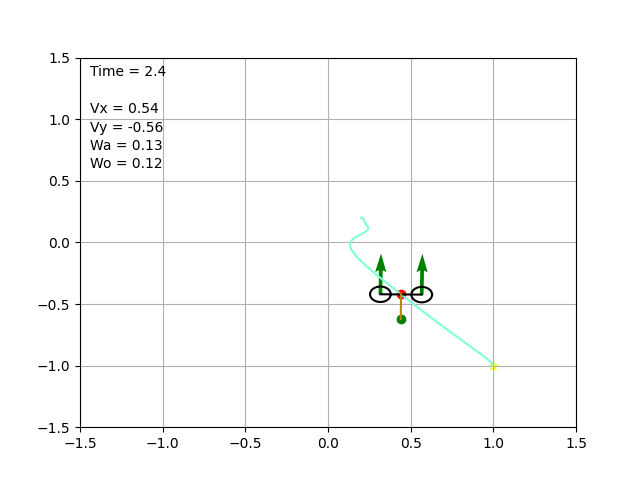
\includegraphics[width=0.9\textwidth]{pictures/ani24.png}
\caption{$t = 2.4s$}
\label{fig:ani24}
\end{figure}

\begin{figure}[H]
\centering
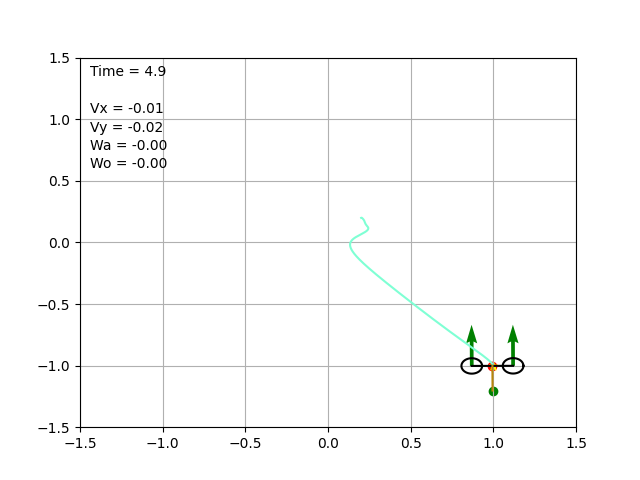
\includegraphics[width=0.9\textwidth]{pictures/ani49.png}
\caption{$t = 4.9s$}
\label{fig:ani49}
\end{figure}